\chapter{Introduction}
  The rise of smartphones and other devices that are capable of using IEEE 802.11 \ac{WLAN} bring along 
  more applications that exhaust any way to reconnect to the internet in order to 
  down an up-load personal data, advertisement or media with a high footprint in storage.
  YouTube, WhatsApp, Facebook and similar apps move high quality images and videos to and from end-users smartphones. 
  Since the number of smartphones in the field are constantly on the rise, this creates an additional strain for
  the backbone and access-links. As users prefer to use WLANs instead of mobile internet-connections due to their costs and limitations with respect to available bandwidth,
  a \ac{WLAN} infrastructure like a \ac{WDS} needs careful planning. Especially use cases like camping sites or large scale deployments (widespread rural areas) with a lot of users
  put high requirements on the \ac{WLAN} backbone. 
  In this paper we consider LANCOM AutoWDS, a \ac{WDS} which implements an easily deployable \ac{WDS} for a set of APs in order to create a wireless 
  infrastructure for a specific area.

  \begin{figure}[h]
    \centering
    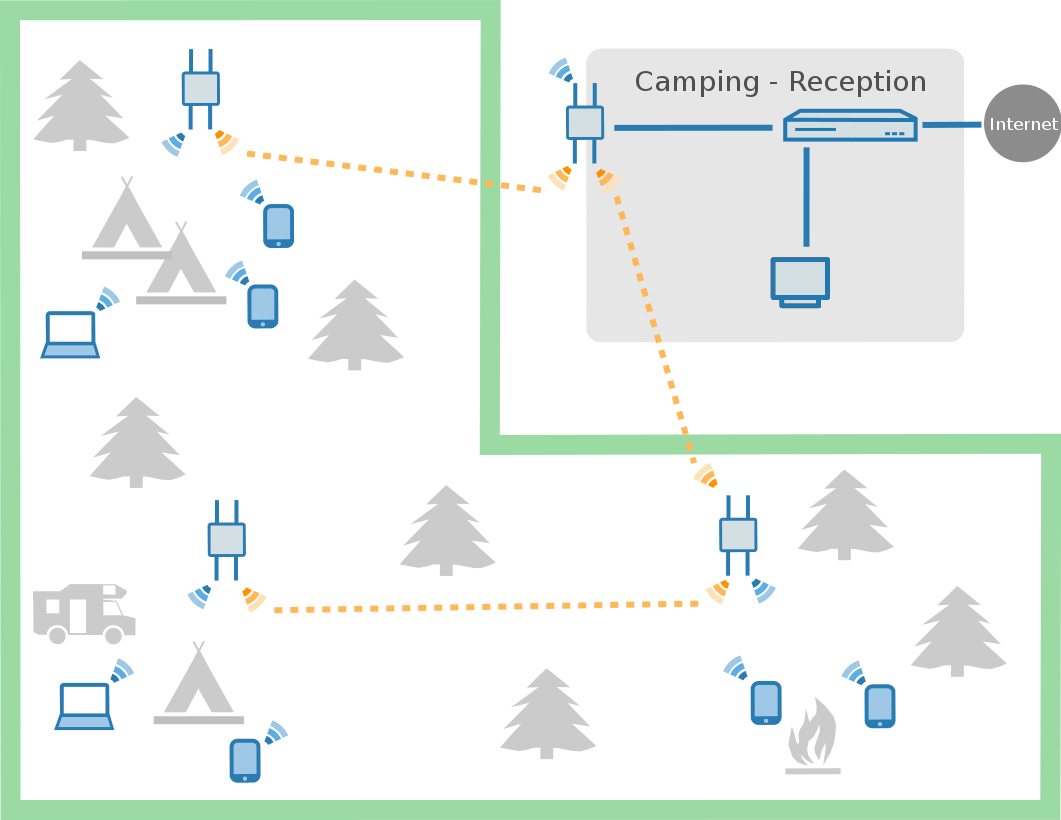
\includegraphics[width=1\columnwidth]{figures/camping.png}
    \caption{WDS deployment at a camping site. Typical scenario for using a \ac{WDS} system instead of wired APs.}
    \label{fig:camping}
  \end{figure}
  
\section{Motivation}
  AutoWDS in its current form does not scale well as throughput performance and an increasing number of connectivity failures quickly bring the system to its limits.
  Our goal is to optimize this system by boosting throughput performance and decreasing the number of occurring simple link failures.
  We want to achieve this by utilizing multiple radios, channels and redundant links (survival paths) for establishing connections among the APs, as using only a single
  channel places artificial limits on the achievable bandwidth.
  This means also we only deal with the physical connectivity (link layer) and are independent of a routing system, which could be placed on top of our solution.
  The problem we face doing this and that our work will elaborate on is that a good selection of links and channels is not trivial even for a moderately sized scenario.
  To tackle this challenge we use centrally run greedy algorithms to give us a better solution to our problem for a static environment.
  
\section{Structure of Thesis}
  At first we will recall terms and concepts used in this work followed by taking a look at the requirements and restrictions a possible solution would have to deal with.
  In Chapter 4, we will then review related work on this field and outline why those approaches have not been pursued.
  Subsequently we will describe our algorithms for choosing a topology, creating backup links and the successive channel assignment, ensued by the implementation of 
  the aforementioned. We will also give an example on how to run the algorithms yourself for a simple scenario.
  In Chapter 7 the procedure is evaluated as a whole in practice and compared to the basic version of AutoWDS.
  Finally we conclude our findings by portraying open issues and identifying promising approaches to pursue.
